\documentclass[journal]{vgtc}                % final (journal style)
%\documentclass[review,journal]{vgtc}         % review (journal style)
%\documentclass[widereview]{vgtc}             % wide-spaced review
%\documentclass[preprint,journal]{vgtc}       % preprint (journal style)

%% Uncomment one of the lines above depending on where your paper is
%% in the conference process. ``review'' and ``widereview'' are for review
%% submission, ``preprint'' is for pre-publication, and the final version
%% doesn't use a specific qualifier.

%% Please use one of the ``review'' options in combination with the
%% assigned online id (see below) ONLY if your paper uses a double blind
%% review process. Some conferences, like IEEE Vis and InfoVis, have NOT
%% in the past.

%% Please note that the use of figures other than the optional teaser is not permitted on the first page
%% of the journal version.  Figures should begin on the second page and be
%% in CMYK or Grey scale format, otherwise, colour shifting may occur
%% during the printing process.  Papers submitted with figures other than the optional teaser on the
%% first page will be refused. Also, the teaser figure should only have the
%% width of the abstract as the template enforces it.

%% These few lines make a distinction between latex and pdflatex calls and they
%% bring in essential packages for graphics and font handling.
%% Note that due to the \DeclareGraphicsExtensions{} call it is no longer necessary
%% to provide the the path and extension of a graphics file:
%% 
\includegraphics{diamondrule} is completely sufficient.
%%
\ifpdf%                                % if we use pdflatex
  \pdfoutput=1\relax                   % create PDFs from pdfLaTeX
  \pdfcompresslevel=9                  % PDF Compression
  \pdfoptionpdfminorversion=7          % create PDF 1.7
  \ExecuteOptions{pdftex}
  \usepackage{graphicx}                % allow us to embed graphics files
  \DeclareGraphicsExtensions{.pdf,.png,.jpg,.jpeg} % for pdflatex we expect .pdf, .png, or .jpg files
\else%                                 % else we use pure latex
  \ExecuteOptions{dvips}
  \usepackage{graphicx}                % allow us to embed graphics files
  \DeclareGraphicsExtensions{.eps}     % for pure latex we expect eps files
\fi%

%% it is recomended to use ``\autoref{sec:bla}'' instead of ``Fig.~\ref{sec:bla}''
\graphicspath{{figures/}{pictures/}{images/}{./}} % where to search for the images


%\usepackage[latin1]{inputenc} % un package
%\usepackage[T1]{fontenc}      % un second package
%\usepackage[francais]{babel}  % un troisième package
\usepackage{microtype}                 % use micro-typography (slightly more compact, better to read)
\PassOptionsToPackage{warn}{textcomp}  % to address font issues with \textrightarrow
\usepackage{textcomp}                  % use better special symbols
\usepackage{mathptmx}                  % use matching math font
\usepackage{times}                     % we use Times as the main font
\renewcommand*\ttdefault{txtt}         % a nicer typewriter font
\usepackage{cite}                      % needed to automatically sort the references
\usepackage{tabu}                      % only used for the table example
\usepackage{booktabs}                 % only used for the table example

%% We encourage the use of mathptmx for consistent usage of times font
%% throughout the proceedings. However, if you encounter conflicts
%% with other math-related packages, you may want to disable it.

%\inputencoding{latin1}
%% In preprint mode you may define your own headline.
%\preprinttext{To appear in IEEE Transactions on Visualization and Computer Graphics.}

%% If you are submitting a paper to a conference for review with a double
%% blind reviewing process, please replace the value ``0'' below with your
%% OnlineID. Otherwise, you may safely leave it at ``0''.
\onlineid{0}

%% declare the category of your paper, only shown in review mode
\vgtccategory{Research}
%% please declare the paper type of your paper to help reviewers, only shown in review mode
%% choices:
%% * algorithm/technique
%% * application/design study
%% * evaluation
%% * system
%% * theory/model
\vgtcpapertype{please specify}

%% Paper title.
\title{Exploring potential causes, consequences and visualizing evolution of major air pollutant emissions over EU28}

%% This is how authors are specified in the journal style

%% Les auteurs 
\author{Jules Sauvinet, Marine Ruiz}
\authorfooter{
%% insert punctuation at end of each item
\item
 Jules Sauvinet is studyingViat Universit\'e Claude Bernard Lyon I. E-mail: contact@julessauvinet.fr
\item
 Marine Ruiz is studying at Universit\'e Claude Bernard Lyon I. E-mail: marine.ruiz@etu.univ-lyon1.fr
}

%other entries to be set up for journal
\shortauthortitle{Biv \MakeLowercase{\textit{et al.}}: Global Illumination for Fun and Profit}
%\shortauthortitle{Firstauthor \MakeLowercase{\textit{et al.}}: Paper Title}

%% Abstract section.
\abstract{Visualization over 12 years des relevés sur des polluants et des relevés sur des données de santé ou autre afin de visualiser ou non, une possible relation entre le polluant et la mesure.
}

%% Keywords that describe your work. Will show as 'Index Terms' in journal
%% please capitalize first letter and insert punctuation after last keyword
\keywords{Air pollution, Ammoniac, Sulphur oxides, Non-methane volatil organic compound, Nitrogen oxides, Particule matters, EU28, eurostats, ecology, health}

%% ACM Computing Classification System (CCS). 
%% See <http://www.acm.org/class/1998/> for details.
%% The ``\CCScat'' command takes four arguments.

\CCScatlist{ % not used in journal version
 \CCScat{K.6.1}{Management of Computing and Information Systems}%
{Project and People Management}{Life Cycle};
 \CCScat{K.7.m}{The Computing Profession}{Miscellaneous}{Ethics}
}

%% Uncomment below to include a teaser figure.
\teaser{
  \centering
  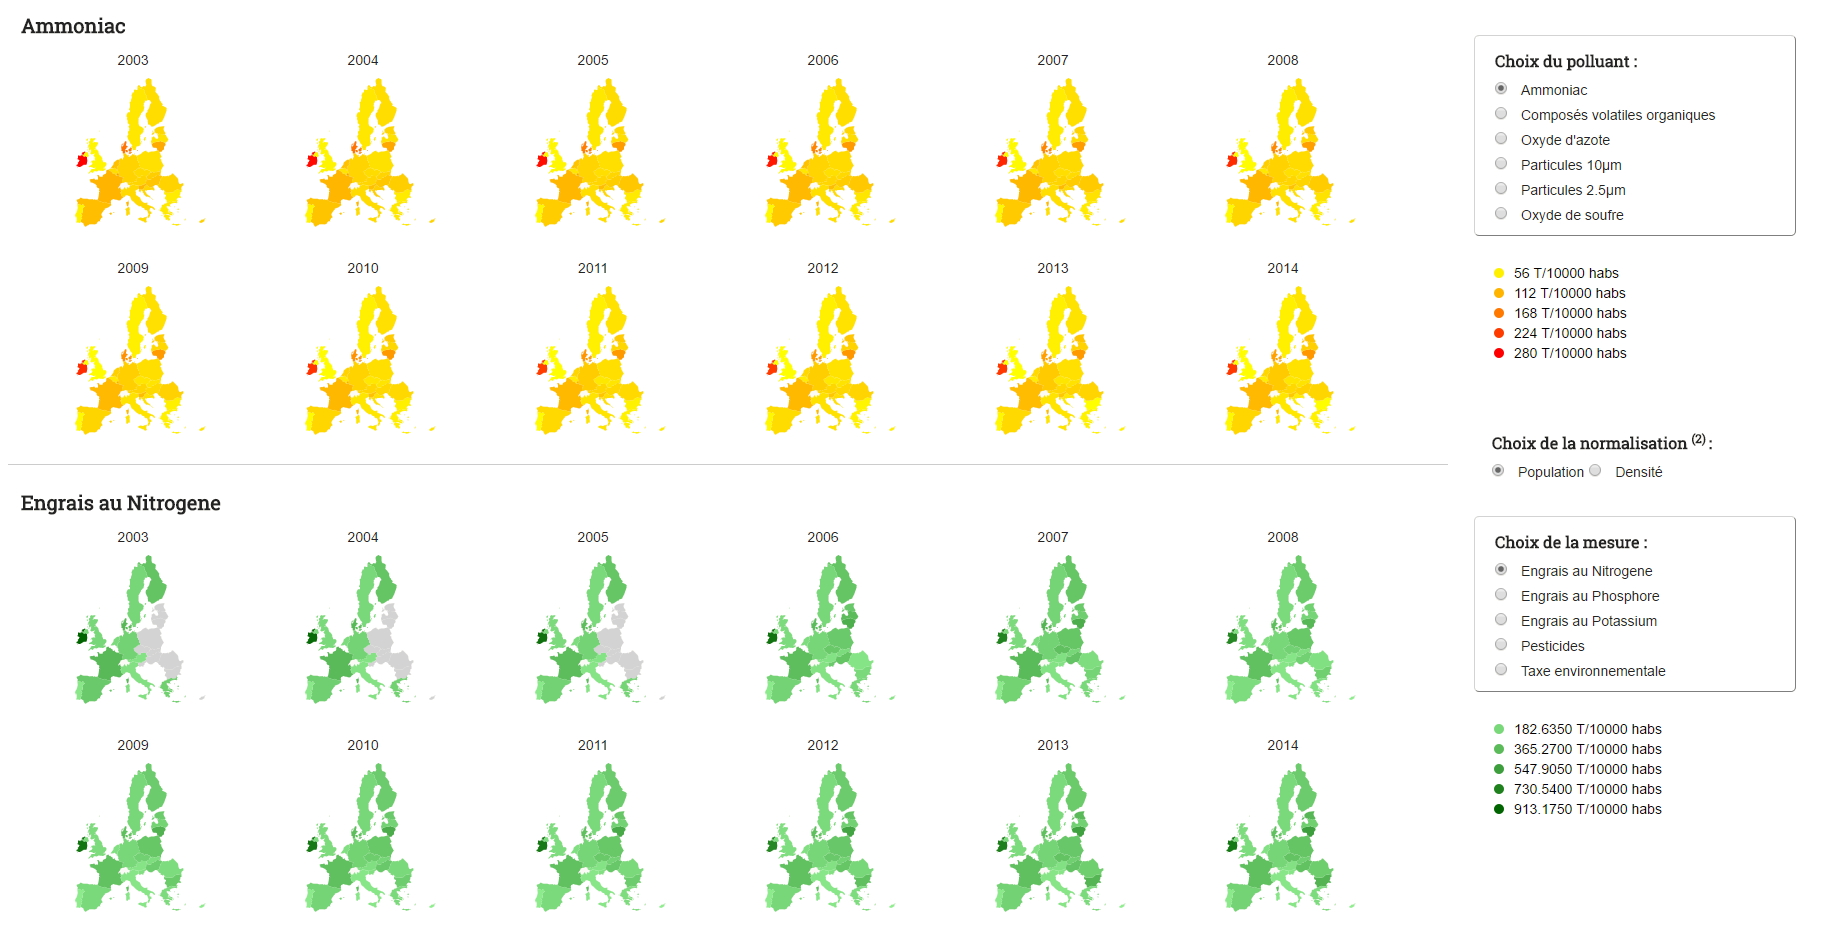
\includegraphics[width=\linewidth]{teaserView}
  \caption{Main view of the visualization: The smallMaps of pollution on the top (the pollutant chose is Ammoniac) and the smallMaps of the mesure below (the mesure chose is the "Engrais azot\'es"')}
	\label{fig:teaser}
}

%% Uncomment below to disable the manuscript note
%\renewcommand{\manuscriptnotetxt}{}

%% Copyright space is enabled by default as required by guidelines.
%% It is disabled by the 'review' option or via the following command:
% \nocopyrightspace

\vgtcinsertpkg

%%%%%%%%%%%%%%%%%%%%%%%%%%%%%%%%%%%%%%%%%%%%%%%%%%%%%%%%%%%%%%%%
%%%%%%%%%%%%%%%%%%%%%% START OF THE PAPER %%%%%%%%%%%%%%%%%%%%%%
%%%%%%%%%%%%%%%%%%%%%%%%%%%%%%%%%%%%%%%%%%%%%%%%%%%%%%%%%%%%%%%%%

\begin{document}

%% The ``\maketitle'' command must be the first command after the
%% ``\begin{document}'' command. It prepares and prints the title block.

%% the only exception to this rule is the \firstsection command
\firstsection{Introduction(1p)}

\maketitle

The emissions of most harmful air pollutants has globally decreased over the past 25 years (see the figure 2 below).
But that doesn't mean that we handle the problem of pollution and that the ...
Some countries have decided to appliquer une politique de r\'eduction, alors que d'autres continuent d'\'emettre des quantit\'es très élevés, posant de sérieux problèmes pour l'environnement et la santé.
Etc ...


\begin{figure}[tb]
 \centering % avoid the use of \begin{center}...\end{center} and use \centering instead (more compact)
 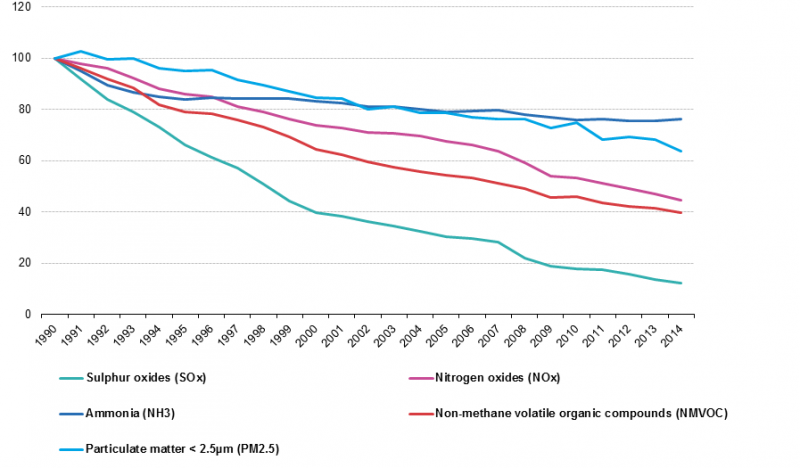
\includegraphics[width=\columnwidth]{decreased_emissions}
 \caption{A visualization of the data from \autoref{tab:vis_papers}. The image is from \cite{Eurostats:2017:VMC} and is in the public domain.}
 \label{fig:pollution decrease}
\end{figure}


Lorem ipsum dolor sit amet, consetetur sadipscing elitr, sed diam
nonumy eirmod tempor invidunt ut labore et dolore magna aliquyam erat,
sed diam voluptua. At vero eos et accusam et justo duo dolores et ea
rebum. Stet clita kasd gubergren, no sea takimata sanctus est Lorem
ipsum dolor sit amet. Lorem ipsum dolor sit amet, consetetur
sadipscing elitr, sed diam nonumy eirmod tempor invidunt ut labore et
dolore magna aliquyam erat, sed diam voluptua. At vero eos et accusam
et justo duo dolores et ea rebum. Stet clita kasd gubergren, no sea
takimata sanctus est Lorem ipsum dolor sit amet. Lorem ipsum dolor sit
amet, consetetur sadipscing elitr, sed diam nonumy eirmod tempor
invidunt ut labore et dolore magna aliquyam erat, sed diam
voluptua. At vero eos et accusam et justo duo dolores et ea
rebum.

Lorem ipsum dolor sit amet, consetetur sadipscing elitr, sed diam
nonumy eirmod tempor invidunt ut labore et dolore magna aliquyam erat,
sed diam voluptua. At vero eos et accusam et justo duo dolores et ea
rebum. Stet clita kasd gubergren, no sea takimata sanctus est Lorem
ipsum dolor sit amet. Lorem ipsum dolor sit amet, consetetur
sadipscing elitr, sed diam nonumy eirmod tempor invidunt ut labore et
dolore magna aliquyam erat, sed diam voluptua. At vero eos et accusam
et justo duo dolores et ea rebum. Stet clita kasd gubergren, no sea
takimata sanctus est Lorem ipsum dolor sit amet. Lorem ipsum dolor sit
amet, consetetur sadipscing elitr, sed diam nonumy eirmod tempor
invidunt ut labore et dolore magna aliquyam erat, sed diam
voluptua. At vero eos et accusam et justo duo dolores et ea
rebum.

Lorem ipsum dolor sit amet, consetetur sadipscing elitr, sed diam
nonumy eirmod tempor invidunt ut labore et dolore magna aliquyam erat,
sed diam voluptua. At vero eos et accusam et justo duo dolores et ea
rebum. Stet clita kasd gubergren, no sea takimata sanctus est Lorem
ipsum dolor sit amet. Lorem ipsum dolor sit amet, consetetur
sadipscing elitr, sed diam nonumy eirmod tempor invidunt ut labore et
dolore magna aliquyam erat, sed diam voluptua. At vero eos et accusam
et justo duo dolores et ea rebum. Stet clita kasd gubergren, no sea
takimata sanctus est Lorem ipsum dolor sit amet. Lorem ipsum dolor sit
amet, consetetur sadipscing elitr, sed diam nonumy eirmod tempor
invidunt ut labore et dolore magna aliquyam erat, sed diam
voluptua. At vero eos et accusam et justo duo dolores et ea
rebum.

Lorem ipsum dolor sit amet, consetetur sadipscing elitr, sed diam
nonumy eirmod tempor invidunt ut labore et dolore magna aliquyam erat,
sed diam voluptua. At vero eos et accusam et justo duo dolores et ea
rebum. Stet clita kasd gubergren, no sea takimata sanctus est Lorem
ipsum dolor sit amet. Lorem ipsum dolor sit amet, consetetur
sadipscing elitr, sed diam nonumy eirmod tempor invidunt ut labore et
dolore magna aliquyam erat, sed diam voluptua. At vero eos et accusam
et justo duo dolores et ea rebum. Stet clita kasd gubergren, no sea
takimata sanctus est Lorem ipsum dolor sit amet. Lorem ipsum dolor sit
amet, consetetur sadipscing elitr, sed diam nonumy eirmod tempor
invidunt ut labore et dolore magna aliquyam erat, sed diam
voluptua. At vero eos et accusam et justo duo dolores et ea
rebum.

Lorem ipsum dolor sit amet, consetetur sadipscing elitr, sed diam
nonumy eirmod tempor invidunt ut labore et dolore magna aliquyam erat,
sed diam voluptua. At vero eos et accusam et justo duo dolores et ea
rebum. Stet clita kasd gubergren, no sea takimata sanctus est Lorem
ipsum dolor sit amet. Lorem ipsum dolor sit amet, consetetur
sadipscing elitr, sed diam nonumy eirmod tempor invidunt ut labore et
dolore magna aliquyam erat, sed diam voluptua. At vero eos et accusam
et justo duo dolores et ea rebum. Stet clita kasd gubergren, no sea
takimata sanctus est Lorem ipsum dolor sit amet. Lorem ipsum dolor sit
amet, consetetur sadipscing elitr, sed diam nonumy eirmod tempor
invidunt ut labore et dolore magna aliquyam erat, sed diam
voluptua. At vero eos et accusam et justo duo dolores et ea
rebum.

Lorem ipsum dolor sit amet, consetetur sadipscing elitr, sed diam
nonumy eirmod tempor invidunt ut labore et dolore magna aliquyam erat,
sed diam voluptua. At vero eos et accusam et justo duo dolores et ea
rebum. Stet clita kasd gubergren, no sea takimata sanctus est Lorem
ipsum dolor sit amet. Lorem ipsum dolor sit amet, consetetur
sadipscing elitr, sed diam nonumy eirmod tempor invidunt ut labore et
dolore magna aliquyam erat, sed diam voluptua. At vero eos et accusam
et justo duo dolores et ea rebum. Stet clita kasd gubergren, no sea
takimata sanctus est Lorem ipsum dolor sit amet. Lorem ipsum dolor sit
amet, consetetur sadipscing elitr, sed diam nonumy eirmod tempor
invidunt ut labore et dolore magna aliquyam erat, sed diam
voluptua. At vero eos et accusam et justo duo dolores et ea
rebum.

Stet clita kasd gubergren, no sea takimata sanctus est Lorem
ipsum dolor sit amet. Lorem ipsum dolor sit amet, consetetur
sadipscing elitr, sed diam nonumy eirmod tempor invidunt ut labore et
dolore magna aliquyam erat, sed diam voluptua. At vero eos et accusam
et justo duo dolores et ea rebum. Stet clita kasd gubergren, no sea
takimata sanctus est Lorem ipsum dolor sit amet. Lorem ipsum dolor sit
amet, consetetur sadipscing elitr, sed diam nonumy eirmod tempor
invidunt ut labore et dolore magna aliquyam erat, sed diam
voluptua. 
%% \section{Introduction} %for journal use above \firstsection{..} instead


\section{Related Work (1p)}

\begin{itemize}
\item Note that each author needs to have a separate entry in author footer on the bottom-left corner of the first page, merging two people (even if from the same institution) is not permitted.
\item The style uses the hyperref package, thus turns references into internal links. We thus recommend to make use of the ``\texttt{\textbackslash autoref\{reference\}}'' call (instead of ``\texttt{Figure\~{}\textbackslash ref\{reference\}}'' or similar) since ``\texttt{\textbackslash autoref\{reference\}}'' turns the entire reference into an internal link, not just the number. Examples: \autoref{fig:sample} and \autoref{tab:vis_papers}.
\item The style automatically looks for image files with the correct extension (eps for regular \LaTeX; pdf, png, and jpg for pdf\LaTeX), in a set of given subfolders (figures/, pictures/, images/). It is thus sufficient to use ``\texttt{\textbackslash includegraphics\{CypressView\}}'' (instead of ``\texttt{\textbackslash includegraphics\{pictures/CypressView.jpg\}}'').
\item For adding hyperlinks and DOIs to the list of references, you can use ``\texttt{\textbackslash bibliographystyle\{abbrv-doi-hyperref-narrow\}}'' (instead of ``\texttt{\textbackslash bibliographystyle\{abbrv\}}''). It uses the doi and url fields in a bib\TeX\ entry and turns the entire reference into a link, giving priority to the doi. The doi can be entered with or without the ``\texttt{http://dx.doi.org/}'' url part. See the examples in the bib\TeX\ file and the bibliography at the end of this template.\\[1em]
\textbf{Note 1:} occasionally (for some \LaTeX\ distributions) this hyper-linked bib\TeX\ style may lead to \textbf{compilation errors} (``\texttt{pdfendlink ended up in different nesting level ...}'') if a reference entry is broken across two pages (due to a bug in hyperref). In this case make sure you have the latest version of the hyperref package (i.\,e., update your \LaTeX\ installation/packages) or, alternatively, revert back to ``\texttt{\textbackslash bibliographystyle\{abbrv-doi-narrow\}}'' (at the expense of removing hyperlinks from the bibliography) and try ``\texttt{\textbackslash bibliographystyle\{abbrv-doi-hyperref-narrow\}}'' again after some more editing.\\[1em]
\textbf{Note 2:} the ``\texttt{-narrow}'' versions of the bibliography style use the font ``PTSansNarrow-TLF'' for typesetting the DOIs in a compact way. This font needs to be available on your \LaTeX\ system. It is part of the \href{https://www.ctan.org/pkg/paratype}{``paratype'' package}, and many distributions (such as MikTeX) have it automatically installed. If you do not have this package yet and want to use a ``\texttt{-narrow}'' bibliography style then use your \LaTeX\ system's package installer to add it. If this is not possible you can also revert to the respective bibliography styles without the ``\texttt{-narrow}'' in the file name.\\[1em]
DVI-based processes to compile the template apparently cannot handle the different font so, by default, the template file uses the \texttt{abbrv-doi} bibliography style but the compiled PDF shows you the effect of the \texttt{abbrv-doi-hyperref-narrow} style.
\textbf{Note 2:} the ``\texttt{-narrow}'' versions of the bibliography style use the font ``PTSansNarrow-TLF'' for typesetting the DOIs in a compact way. This font needs to be available on your \LaTeX\ system. It is part of the \href{https://www.ctan.org/pkg/paratype}{``paratype'' package}, and many distributions (such as MikTeX) have it automatically installed. If you do not have this package yet and want to use a ``\texttt{-narrow}'' bibliography style then use your \LaTeX\ system's package installer to add it. If this is not possible you can also revert to the respective bibliography styles without the ``\texttt{-narrow}'' in the file name.\\[1em]
DVI-based processes to compile the template apparently cannot handle the different font so, by default, the template file uses the \texttt{abbrv-doi} bibliography style but the compiled PDF shows you the effect of the \texttt{abbrv-doi-hyperref-narrow} style.
\end{itemize}

Lorem ipsum dolor sit amet, consetetur sadipscing elitr, sed diam
nonumy eirmod tempor invidunt ut labore et dolore magna aliquyam erat,
sed diam voluptua. At vero eos et accusam et justo duo dolores et ea
rebum. Stet clita kasd gubergren, no sea takimata sanctus est Lorem
ipsum dolor sit amet. Lorem ipsum dolor sit amet, consetetur
sadipscing elitr, sed diam nonumy eirmod tempor invidunt ut labore et
dolore magna aliquyam erat, sed diam voluptua. At vero eos et accusam
et justo duo dolores et ea rebum. Stet clita kasd gubergren, no sea
takimata sanctus est Lorem ipsum dolor sit amet. Lorem ipsum dolor sit
amet, consetetur sadipscing elitr, sed diam nonumy eirmod tempor
invidunt ut labore et dolore magna aliquyam erat, sed diam
voluptua. At vero eos et accusam et justo duo dolores et ea
rebum.

Lorem ipsum dolor sit amet, consetetur sadipscing elitr, sed diam
nonumy eirmod tempor invidunt ut labore et dolore magna aliquyam erat,
sed diam voluptua. At vero eos et accusam et justo duo dolores et ea
rebum. Stet clita kasd gubergren, no sea takimata sanctus est Lorem
ipsum dolor sit amet. Lorem ipsum dolor sit amet, consetetur
sadipscing elitr, sed diam nonumy eirmod tempor invidunt ut labore et
dolore magna aliquyam erat, sed diam voluptua. At vero eos et accusam
et justo duo dolores et ea rebum. Stet clita kasd gubergren, no sea
takimata sanctus est Lorem ipsum dolor sit amet. Lorem ipsum dolor sit
amet, consetetur sadipscing elitr, sed diam nonumy eirmod tempor
invidunt ut labore et dolore magna aliquyam erat, sed diam
voluptua. At vero eos et accusam et justo duo dolores et ea
rebum.

Lorem ipsum dolor sit amet, consetetur sadipscing elitr, sed diam
nonumy eirmod tempor invidunt ut labore et dolore magna aliquyam erat,
sed diam voluptua. At vero eos et accusam et justo duo dolores et ea
rebum. Stet clita kasd gubergren, no sea takimata sanctus est Lorem
ipsum dolor sit amet. Lorem ipsum dolor sit amet, consetetur
sadipscing elitr, sed diam nonumy eirmod tempor invidunt ut labore et
dolore magna aliquyam erat, sed diam voluptua. At vero eos et accusam
et justo duo dolores et ea rebum. Stet clita kasd gubergren, no sea
takimata sanctus est Lorem ipsum dolor sit amet. Lorem ipsum dolor sit
amet, consetetur sadipscing elitr, sed diam nonumy eirmod tempor
invidunt ut labore et dolore magna aliquyam erat, sed diam
voluptua. At vero eos et accusam et justo duo dolores et ea
rebum.

Lorem ipsum dolor sit amet, consetetur sadipscing elitr, sed diam
nonumy eirmod tempor invidunt ut labore et dolore magna aliquyam erat,
sed diam voluptua. At vero eos et accusam et justo duo dolores et ea
rebum. Stet clita kasd gubergren, no sea takimata sanctus est Lorem
ipsum dolor sit amet. Lorem ipsum dolor sit amet, consetetur
sadipscing elitr, sed diam nonumy eirmod tempor invidunt ut labore et
dolore magna aliquyam erat, sed diam voluptua. At vero eos et accusam
et justo duo dolores et ea rebum. Stet clita kasd gubergren, no sea
takimata sanctus est Lorem ipsum dolor sit amet. Lorem ipsum dolor sit
amet, consetetur sadipscing elitr, sed diam nonumy eirmod tempor
invidunt ut labore et dolore magna aliquyam erat, sed diam
voluptua. At vero eos et accusam et justo duo dolores et ea
rebum.
Lorem ipsum dolor sit amet, consetetur sadipscing elitr, sed diam
nonumy eirmod tempor invidunt ut labore et dolore magna aliquyam erat,
sed diam voluptua. At vero eos et accusam et justo duo dolores et ea
rebum. Stet clita kasd gubergren, no sea takimata sanctus est Lorem
ipsum dolor sit amet. Lorem ipsum dolor sit amet, consetetur
sadipscing elitr, sed diam nonumy eirmod tempor invidunt ut labore et
dolore magna aliquyam erat, sed diam voluptua. At vero eos et accusam
et justo duo dolores et ea rebum. Stet clita kasd gubergren, no sea
takimata sanctus est Lorem ipsum dolor sit amet. Lorem ipsum dolor sit
amet, consetetur sadipscing elitr, sed diam nonumy eirmod tempor
invidunt ut labore et dolore magna aliquyam erat, sed diam
voluptua. 

Lorem ipsum dolor sit amet, consetetur sadipscing elitr, sed diam
nonumy eirmod tempor invidunt ut labore et dolore magna aliquyam erat,
sed diam voluptua. At vero eos et accusam et justo duo dolores et ea
rebum. Stet clita kasd gubergren, no sea takimata sanctus est Lorem
ipsum dolor sit amet. Lorem ipsum dolor sit amet, consetetur
sadipscing elitr, sed diam nonumy eirmod tempor invidunt ut labore et
dolore magna aliquyam erat, sed diam voluptua. At vero eos et accusam
et justo duo dolores et ea rebum. Stet clita kasd gubergren, no sea
takimata sanctus est Lorem ipsum dolor sit amet. Lorem ipsum dolor sit
amet, consetetur sadipscing elitr, sed diam nonumy eirmod tempor
invidunt ut labore et dolore magna aliquyam erat, sed diam
voluptua. At vero eos et accusam et justo duo dolores et ea
rebum.

\section{Project Description (2p)}

	\subsection{Visualization description}
	
	\begin{itemize}
		\item Les 12 maps polluants avec la légende
			\begin{itemize}
				\item Si on choisit un autre polluant dans la liste, les maps se mettent à jour
				\item Permet le dynamisme de la vizu des polluants.
			\end{itemize}
			
		\item Les 12 maps de mesure avec la légende
			\begin{itemize}
				\item Si on choisit une autre mesure dans la liste, les maps se mettent à jour et on affiche les maps uniquement avec les années sur lesquelles nous avons des données et polluant et mesure sélectionnés dans la limite de 12 années
				\item Permet le dynamisme de la vizu des mesures.
				\item permet de maximiser l’information grâce aux années dynamique, on s’adapte aux données et non l’inverse, on n’affiche jamais de map toute grise
				\item Si on choisit un autre polluant, la liste des mesures est modifié pour proposer des mesures intéressantes à comparer avec le polluant
				\item Permet de maximiser les comparaisons, on enlève ce qui n’est pas pertinent pour que l’utilisateur ne perde pas de temps inutilement
			\end{itemize}

		\item la normalisation des données
			\begin{itemize}
				\item Si on change la normalisation des données, les 24 maps et la légende se mettent à jour
				\item Les pays les plus peuplé pollue plus, il faut faire un pourcentage
			\end{itemize}
		
		
		\item l’affichage des valeurs
			\begin{itemize}
				\item Quand on passe la souris sur un pays de n’importe quelle map, polluant comme mesure, le nom du pays apparaît et les années sont remplacées par la valeur sur les 24 maps (les années où il n’y pas de données pour le pays, rien ne s’affiche)
				\item L’agencement de la vizu permet dès le premier regard de se faire une idée de la corrélation mais afficher les valeurs sur les 24 maps permet de faire un idée rapide de l’évolution de la donnée. On peut aussi comparer son évolution avec l’autre donnée (corrélation, anti-corrélation, rien)
				\item on a une liste de tous les pays qui sont pris en compte
				\item on peut cocher ou décocher tous les pays de la liste suivant si l’on veut les visualiser ou non. 		
				\item La légende se met à jour si cela est nécessaire. Le pays devient gris sur toutes les maps, et passer la souris dessus ne change rien à la Vizu.
				\item certains pays biaisent la légende en ayant des valeurs extrêmes. On peut donc choisir de ne pas prendre en compte ce pays et ainsi obtenir une échelle plus raffinée. On peut de ce fait faire une coloration de seulement quelques pays si on le souhaite
			\end{itemize}
			
	\end{itemize}

	\subsection{Choice of the measures}
	We chose 18 measures that we considered relevant regarding the pollutants we selected : 
		\begin{itemize}
		\item Cancer death (Morts de cancers)
		\item Pesticides (Pesticides)
		\item Nitrogen fertilizers
		\item Potassium fertilizers
		\item Phosphore fertilizers
		\item Environmental tax (Taxe environnementale)
		\item Transport tax (Taxe transport)
		\item Primary production of electricity (Production primaire d\'énergie)
		\item Primary production of renewable electricity (Production primaire d\'énergie renouvelable)
		\item Primary production of oil (Production primaire de pétrole)
		\item Primary production of gas (Production primaire de gaz)
		\item Primary production of coal (Production primaire de charbon)
		\item Nuclear heat (Production primaire d'énergie nucleaire)
		\item Heart diseases deaths (Morts de maladies cardiaques)
		\item Diesel motor cars (Moteurs de voitures diesel)
		\item Petrol motor cars (Moteurs de voitures pétrole)
		\item Length of hospitals stays for lung diseases (Jours d\'hospitalisation pour maladie pulmmonaire)
		\end{itemize}
		
		We first searched for each pollutants the possible causes and consequences of the emissions. Then we tried to find adapted measures in the database for eurostats.\\
		For the Ammoniac pollutant, we identified that the major sector produces rejects was the agriculture (figure 3).\\
		Etc.. Pesticides et engrais.\\
		
		For the particules matters pollutants (PM2.5 and PM10), we identified that the major sector produces rejects cas diesel combustion ...\\
		.\\
		Etc.. Pesticides et engrais.\\
		
		Since countries are specialized in producing certains type d'énergie etc.. 
	
Lorem ipsum dolor sit amet, consetetur sadipscing elitr, sed diam
nonumy eirmod tempor invidunt ut labore et dolore magna aliquyam erat,
sed diam voluptua. At vero eos et accusam et justo duo dolores et ea
rebum. Stet clita kasd gubergren, no sea takimata sanctus est Lorem
ipsum dolor sit amet. Lorem ipsum dolor sit amet, consetetur
sadipscing elitr, sed diam nonumy eirmod tempor invidunt ut labore et
dolore magna aliquyam erat, sed diam voluptua. At vero eos et accusam
et justo duo dolores et ea rebum. Stet clita kasd gubergren, no sea
takimata sanctus est Lorem ipsum dolor sit amet. Lorem ipsum dolor sit
amet, consetetur sadipscing elitr, sed diam nonumy eirmod tempor
invidunt ut labore et dolore magna aliquyam erat, sed diam
voluptua. At vero eos et accusam et justo duo dolores et ea
rebum.

Lorem ipsum dolor sit amet, consetetur sadipscing elitr, sed diam
nonumy eirmod tempor invidunt ut labore et dolore magna aliquyam erat,
sed diam voluptua. At vero eos et accusam et justo duo dolores et ea
rebum. Stet clita kasd gubergren, no sea takimata sanctus est Lorem
ipsum dolor sit amet. Lorem ipsum dolor sit amet, consetetur
sadipscing elitr, sed diam nonumy eirmod tempor invidunt ut labore et
dolore magna aliquyam erat, sed diam voluptua. At vero eos et accusam
et justo duo dolores et ea rebum. Stet clita kasd gubergren, no sea
takimata sanctus est Lorem ipsum dolor sit amet. Lorem ipsum dolor sit
amet, consetetur sadipscing elitr, sed diam nonumy eirmod tempor
invidunt ut labore et dolore magna aliquyam erat, sed diam
voluptua. At vero eos et accusam et justo duo dolores et ea
rebum.

Lorem ipsum dolor sit amet, consetetur sadipscing elitr, sed diam
nonumy eirmod tempor invidunt ut labore et dolore magna aliquyam erat,
sed diam voluptua. At vero eos et accusam et justo duo dolores et ea
rebum. Stet clita kasd gubergren, no sea takimata sanctus est Lorem
ipsum dolor sit amet. Lorem ipsum dolor sit amet, consetetur
sadipscing elitr, sed diam nonumy eirmod tempor invidunt ut labore et
dolore magna aliquyam erat, sed diam voluptua. At vero eos et accusam
et justo duo dolores et ea rebum. Stet clita kasd gubergren, no sea
takimata sanctus est Lorem ipsum dolor sit amet. Lorem ipsum dolor sit
amet, consetetur sadipscing elitr, sed diam nonumy eirmod tempor
invidunt ut labore et dolore magna aliquyam erat, sed diam
voluptua. At vero eos et accusam et justo duo dolores et ea
rebum.

Lorem ipsum dolor sit amet, consetetur sadipscing elitr, sed diam
nonumy eirmod tempor invidunt ut labore et dolore magna aliquyam erat,
sed diam voluptua. At vero eos et accusam et justo duo dolores et ea
rebum. Stet clita kasd gubergren, no sea takimata sanctus est Lorem
ipsum dolor sit amet. Lorem ipsum dolor sit amet, consetetur
sadipscing elitr, sed diam nonumy eirmod tempor invidunt ut labore et
dolore magna aliquyam erat, sed diam voluptua. At vero eos et accusam
et justo duo dolores et ea rebum. Stet clita kasd gubergren, no sea
takimata sanctus est Lorem ipsum dolor sit amet. Lorem ipsum dolor sit
amet, consetetur sadipscing elitr, sed diam nonumy eirmod tempor
invidunt ut labore et dolore magna aliquyam erat, sed diam
voluptua. At vero eos et accusam et justo duo dolores et ea
rebum.
Lorem ipsum dolor sit amet, consetetur sadipscing elitr, sed diam
nonumy eirmod tempor invidunt ut labore et dolore magna aliquyam erat,
sed diam voluptua. At vero eos et accusam et justo duo dolores et ea
rebum. Stet clita kasd gubergren, no sea takimata sanctus est Lorem
ipsum dolor sit amet. Lorem ipsum dolor sit amet, consetetur
sadipscing elitr, sed diam nonumy eirmod tempor invidunt ut labore et
dolore magna aliquyam erat, sed diam voluptua. At vero eos et accusam
et justo duo dolores et ea rebum. Stet clita kasd gubergren, no sea
takimata sanctus est Lorem ipsum dolor sit amet. Lorem ipsum dolor sit
amet, consetetur sadipscing elitr, sed diam nonumy eirmod tempor
invidunt ut labore et dolore magna aliquyam erat, sed diam
voluptua. At vero eos et accusam et justo duo dolores et ea
rebum.
Lorem ipsum dolor sit amet, consetetur sadipscing elitr, sed diam
nonumy eirmod tempor invidunt ut labore et dolore magna aliquyam erat,
sed diam voluptua. At vero eos et accusam et justo duo dolores et ea
rebum. Stet clita kasd gubergren, no sea takimata sanctus est Lorem
ipsum dolor sit amet. Lorem ipsum dolor sit amet, consetetur
sadipscing elitr, sed diam nonumy eirmod tempor invidunt ut labore et
dolore magna aliquyam erat, sed diam voluptua. At vero eos et accusam
et justo duo dolores et ea rebum. Stet clita kasd gubergren, no sea
takimata sanctus est Lorem ipsum dolor sit amet. Lorem ipsum dolor sit
amet, consetetur sadipscing elitr, sed diam nonumy eirmod tempor
invidunt ut labore et dolore magna aliquyam erat, sed diam
voluptua. At vero eos et accusam et justo duo dolores et ea
rebum.

\section{Evaluation (optionnel)}

	On pourrait dire qu'on l'a fait tester à notre famille/amis c'est deja ca.\\
	~\\
	Lorem ipsum dolor sit amet, consetetur sadipscing elitr, sed diam
	nonumy eirmod tempor invidunt ut labore et dolore magna aliquyam erat,
	sed diam voluptua. At vero eos et accusam et justo duo dolores et ea
	rebum. Stet clita kasd gubergren, no sea takimata sanctus est Lorem
	ipsum dolor sit amet. Lorem ipsum dolor sit amet, consetetur
	sadipscing elitr, sed diam nonumy eirmod tempor invidunt ut labore et
	dolore magna aliquyam erat, sed diam
	voluptua~\cite{Kitware:2003,Max:1995:OMF}. At vero eos et accusam et
	justo duo dolores et ea rebum. Stet clita kasd gubergren, no sea
	takimata sanctus est Lorem ipsum dolor sit amet. Lorem ipsum dolor sit
	amet, consetetur sadipscing elitr, sed diam nonumy eirmod tempor
	invidunt ut labore et dolore magna aliquyam erat, sed diam
	voluptua. At vero eos et accusam et justo duo dolores et ea
	rebum. Stet clita kasd gubergren, no sea takimata sanctus est.

\section{Discussion (~½p)}

	Les limites rencontrées / nos idées non développées / améliorations possibles :

	\begin{itemize}
		\item Problème de compatibilité entre nos deux ordinateurs pour visualiser le projet (pas le temps)		
		\item Quand on clique sur pays, un graphique apparaît avec cette fois-ci toutes les années (sans limite de nombre), les courbes d’évolution de la donnée polluant et de la donnée mesures.
		\item → cela aurait pu permettre de mieux visualiser la corrélation entre les deux données 
		\item Quand on clique sur un pays, un tableau des valeurs pour tous les autres pays pour l’année courante
		\item Cela aurait pu permettre de mieux visualiser le pays ciblé en fonction des autres de façon plus précise que par la coloration
		\item intégrer la notion de respect de normes écologiques pour mettre en évidence les pays qui ne la respectent pays
		\item plus de polluants intéressants (il aurait fallu interroger des personnes avec une connaissance approfondie du sujet) (ozone…) et plus de mesures (idem) (de santé)
		\item → cela aurait pu permettre d’avoir une liste de polluants et de mesures associés plus que pertinents
		\item → ATTENTION LES DONNÉES NE SONT PAS TOUJOURS DISPONIBLES / PUBLICS NON PLUS
		\item possibilité de naviguer au travers de toutes les années disponibles sur la combinaison polluant/mesure avec un slider d’intervalles de 12 années
		\item passer d’années en mois (en gardant un slider pour naviguer sur les années) et afficher l’évolution sur une seule année et faire des corrélations sur les saisons  
		\item → mais données non compatibles à ce jour
		\item passer en NUTS2 pour plus de précision 
		\item → plus précis, mais trop précis par rapport à la taille de la SmallMap qu’il faudrait de ce fait agrandir et donc réduire le nombre d’années affichées = compromis
	\end{itemize}

\section{Conclusion}

Lorem ipsum dolor sit amet, consetetur sadipscing elitr, sed diam
nonumy eirmod tempor invidunt ut labore et dolore magna aliquyam erat,
sed diam voluptua. At vero eos et accusam et justo duo dolores et ea
rebum. Stet clita kasd gubergren, no sea takimata sanctus est Lorem
ipsum dolor sit amet. Lorem ipsum dolor sit amet, consetetur
sadipscing elitr, sed diam nonumy eirmod tempor invidunt ut labore et
dolore magna aliquyam erat, sed diam voluptua. At vero eos et accusam
et justo duo dolores et ea rebum. Stet clita kasd gubergren, no sea
takimata sanctus est Lorem ipsum dolor sit amet. Lorem ipsum dolor sit
amet, consetetur sadipscing elitr, sed diam nonumy eirmod tempor
invidunt ut labore et dolore magna aliquyam erat, sed diam
voluptua. At vero eos et accusam et justo duo dolores et ea
rebum.


%% if specified like this the section will be committed in review mode
\acknowledgments{
The authors wish to thank your mother and your sister. This work was supported in part by
a grant from myass.}

%\bibliographystyle{abbrv}
\bibliographystyle{abbrv-doi}
%\bibliographystyle{abbrv-doi-narrow}
%\bibliographystyle{abbrv-doi-hyperref}
%\bibliographystyle{abbrv-doi-hyperref-narrow}
\bibliography{air_pollution_EU28}
\end{document}

